\documentclass[a0paper,portrait]{baposter}

\usepackage{color}
\usepackage{graphicx}
\usepackage{setspace}
% \usepackage[firstinits=true]{biblatex}

\newcommand{\kmer}{$k$-mer\ }
\newcommand{\kmers}{$k$-mers\ }
\newcommand{\fpkm}{\ensuremath{\hbox{\textit{FPKM}}}\ }
\newcommand{\Tophat}{\textit{TopHat}\ }
\newcommand{\Cufflinks}{\textit{Cufflinks}\ }
\newcommand{\Electus}{\textit{Electus}\ }

\bibliographystyle{abbrv}

%%% Color Definitions %%%%%%%%%%%%%%%%%%%%%%%%%%%%%%%%%%%%%%%%%%%%%%%%%%%%%%%%%

%\definecolor{headercol}{RGB}{0,0,0}
%\definecolor{headerfontcol}{RGB}{255,255,255}
\definecolor{headercol}{RGB}{64,64,200}
\definecolor{headerfontcol}{RGB}{255,255,255}
\definecolor{bordercol}{RGB}{0,0,0}
\definecolor{graphred}{RGB}{255,0,0}
\definecolor{graphblue}{RGB}{0,0,255}
\definecolor{graphgreen}{RGB}{0,255,0}

\begin{document}
\begin{poster}{
    grid=false,
    columns=3,
    headerheight=0.12\textheight,
    background=none,
    headerborder=closed,
    borderColor=bordercol,
    headerColorOne=headercol,
    headerborder=closed,
    headerFontColor=headerfontcol,
    headershape=smallrounded,
    headershade=plain,
    headerfont=\bf\Large\textsc,
    textborder=rectangle,
    boxshade=none
}
% Eye catcher
{
    Eye catcher
}
% Title
{
\bf\textsc{Electus: a lightweight tool for extracting targeted sets of reads from large NGS data sets}\vspace{0.2em}
}
% Authors
{
\textsc\large{Jeremy Wazny, Thomas Conway, Andrew Bromage, Geoffrey MacIntyre, Bryan Beresford-Smith}

\textsc\large{NICTA$^{*}$ Victoria Research Laboratory \& \\ Dept. of Computing and Information Systems, The University of Melbourne, Parkville, Australia}
}
% Institution logo(s)
{

\includegraphics[width=0.075\linewidth]{logos_vert}
%\includegraphics[width=0.1\linewidth]{logo_nicta2}
%\includegraphics[width=0.05\linewidth]{logo_unimelb2}
}

\begin{posterbox}[name=problem,column=0,row=0]{Problem}
Second Generation Sequencing enables the collection of large quantities of sequence data.
While such data sets are incredibly rich, often researchers are interested in answering specific questions about the data.
Typically, a researcher with 100s of gigabytes of RNA-Seq data may be interested in SNPs and relative expression for only a small number of specific genes.
In such a scenario, it is unnecessarily time consuming to process the entire data set against a whole reference set of genes, only to discard most of the analysis products.

Furthermore, to answer some questions detailed alignments may not be necessary. For instance, to determine relative gene expression, simply extracting and counting the relevant subset of reads may be sufficient.
While other questions may require assembly or alignment to be performed, applying these algorithms to a subset of the total collection of reads can yield substantial computational savings, provided that the subset can be extracted efficiently.
\end{posterbox}

\begin{posterbox}[name=filtering,column=0,below=problem]{Filter reads}
We have developed a tool, \Electus, which allows the user to quickly and sensitively extract a relevant selection of reads. Using our previously published representation for \textit{k}-mer sets \cite{ConwayBromage2011}, our tool uses a \textit{k}-mer decomposition of the reference sequence(s) of interest to yield crude but effective read alignments.

We have tested this approach in the analysis of a number of prostate cancer RNA-Seq data sets,
and show that for analysis targeted to the genes involved in known fusions,
Electus enables us to efficiently produce files containing just those reads that map to the nominated genes, allowing the \fpkm \cite{trapnell2010} measure of gene expression to be computed quickly.
\end{posterbox}

\begin{posterbox}[name=fpkm,column=0,below=filtering]{Estimate \fpkm}
We have used \Electus to efficiently extract subsets of reads with \kmers in common with specific genes, 
allowing us to quickly produce an estimate of \fpkm.
Because \Electus typically overestimates subsets (especially for low $k$), incorporating it into a pipeline before further filtering with a more specific aligner, e.g. \textit{TopHat}, is conservative.

\vspace{1.0em}
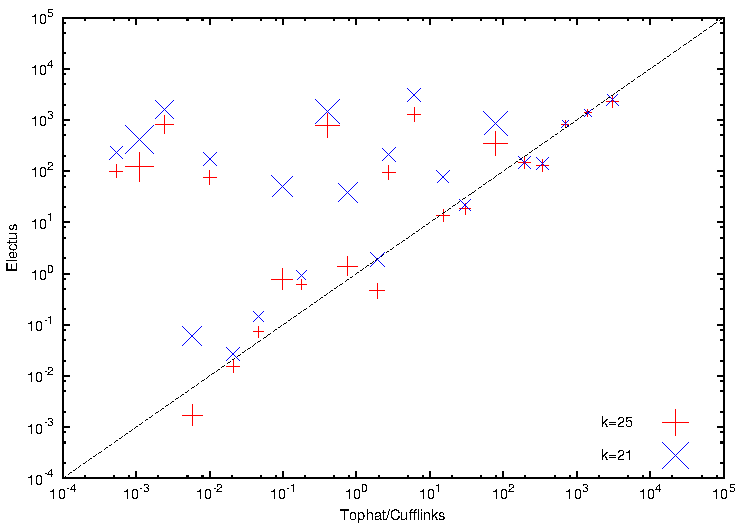
\includegraphics[width=\linewidth]{fpkm-vs_cuff}
\begin{center}
\footnotesize
Comparison of \fpkm value calculated by \Tophat \cite{tophat}-then-\Cufflinks \cite{cufflinks} and \Electus at: \textcolor{red}{$k = 25$} and \textcolor{blue}{$k = 21$}.
Tick size corresponds to gene sequence length.
\end{center}

\end{posterbox}

\begin{posterbox}[name=graphs,column=1,row=0]{Reduce complexity}
To illustrate the reduction in complexity of the data after filtering, we have rendered the \textit{de Bruijn} graph of 
a set of reads before and after filtering for \kmers belonging to a pair of genes known to have fused in a cancer transcriptome.
Each graph edge belongs to one of: \textcolor{graphblue}{gene X}, \textcolor{graphred}{gene Y}, the \textcolor{graphgreen}{fusion sequence}, or some other incidental sequence.

In both cases, only the subset of the graph within 15 levels of branching of the fusion site is shown.

\vspace{1.0em}
\begin{center}
\includegraphics[width=0.9\linewidth]{all-t1-r15lp}
\footnotesize
Graph of all pairs.
\end{center}

\vspace{1.0em}
\begin{center}
\includegraphics[width=0.9\linewidth]{sub-t1-r15lp}
\footnotesize
Graph of pairs with \textcolor{graphblue}{X},\textcolor{graphred}{Y} and \textcolor{graphgreen}{fusion} \kmers.
\end{center}

\end{posterbox}

\begin{posterbox}[name=runtime,column=1,below=graphs]{Reduce runtime}
When only a well-defined subset of reads is required, \Electus can be run to home in quickly 
on that subset, reducing the runtime of subsequent steps in the pipeline.

\vspace{-0.5em}

\begin{center}
\begin{tabular}[]{lll}
            & \bf{Time} \\
\bf{Electus}     &  1h 9m 49s \\
~~~\bf{then TopHat-Fusion} & 1h 29m 11s \\
\bf{TopHat-Fusion} & 2d, 4h 53m 37s \\
\end{tabular}

\vspace{0.5em}

\footnotesize
Comparison of runtimes when only reads corresponding to a set of suspected fusions is extracted. 
The full data set contains $\sim99\times10^6$ RNA-Seq read pairs.
\end{center}

\end{posterbox}

\begin{posterbox}[name=usage,column=2,row=0]{Usage}
\Electus works by building the set of \kmers belonging to a collection of references 
and then classifying reads based on whether they share \kmers
with sufficiently many references. 

To extract a subset of reads which coincide with a reference FASTA file:

\hspace{0.1em} {\tt\footnotesize electus classify --ref-fasta X.fa $...$}

For longer ({\footnotesize$>\sim$}10 Mb) references, build an index:

\hspace{0.1em} {\tt\footnotesize electus index --ref-fasta Y.fa --prefix Y $...$}

\hspace{0.1em} {\tt\footnotesize electus classify --ref-index Y $...$}

Or combine the two.

\hspace{0.1em} {\tt\footnotesize electus classify --ref-fasta X.fa --ref-index Y $...$}

%The individual reads are partitioned into separate files according to whether
%they share enough \kmers with references.
%The ordering of reads in pairs split across files is maintained.
\end{posterbox}

\begin{posterbox}[name=kmers,column=2,below=usage]{Sparse \kmer sets}

\Electus uses a sparse \kmer set data structure based on our compressed bitmap representation\ \cite{ConwayBromage2011}
used previously to encode de Bruijn graphs for {\em de novo} assembly.
This array contains $4^k$ entries: $1$ when the corresponding \kmer is present in the set, and $0$ otherwise.
The theoretical minimum bits required to {\em exactly} represent an array of $m$ entries is $\mathit{log}_2 {{4^k}\choose{m}}$.

%\vspace{-2.0em}
\begin{center}
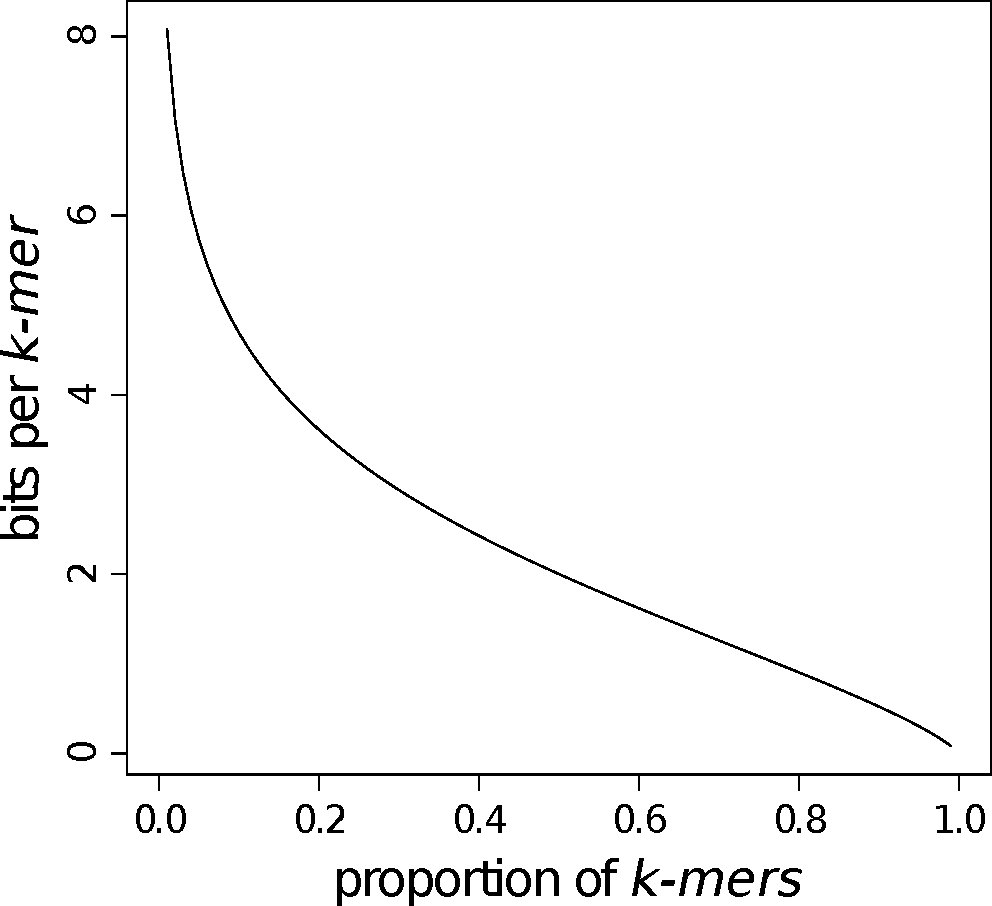
\includegraphics[scale=0.32]{bits-per-kmer-theory}
\end{center}

%To store the set of $\sim2,375$ million $25$-mers of the {\em hg19} human reference genome requires at least $\sim5.6$ GB of storage.
%A straightforward 2 bits-per-base encoding of the \kmers would take $\sim13.8$ GB of space.
%By comparison, our representation achieves this in $\sim7.7$ GB.

\vspace{-1.0em}

The nature of the succinct representation ensures that the bits/\kmer stored
is guaranteed to monotonically decrease as the number of \kmers increases.
Furthermore, unlike probabilistic data structures, it is a {\em self-index} 
and captures the exact set of \kmers {\em precisely}, with no false positives.
\vspace{-2.5em}

\begin{center}
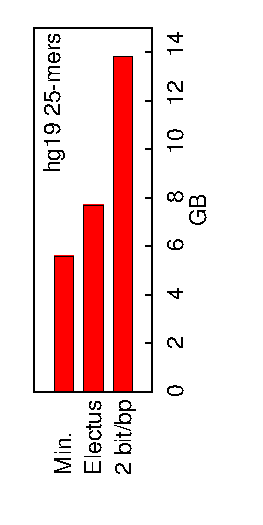
\includegraphics[angle=-90,scale=0.65]{hg19size}
\end{center}
\vspace{-2.5em}
\end{posterbox}

\begin{posterbox}[name=refs,column=2,row=0.725]{References}
\vspace{0.5em}
\begin{spacing}{0.1}
\footnotesize
\renewcommand{\refname}{\vspace{-0.8em}}
\bibliography{poster}
$^{*}$ NICTA is funded by the Australian Government as represented by the Department of Broadband, Communications and the Digital Economy and the Australian Research Council through the ICT Centre of Excellence program.
\end{spacing}
\end{posterbox}

\end{poster}
\end{document}
